\section{Ejercicio 3}
\label{sec:ej3}


\subsection{Consigna}

\begin{enumerate}
	\setcounter{enumi}{2} % Fuerza a que la lista empiece en el número 3
	\item Implemente una red de Hopfield '82 que aprenda patrones pseudo-aleatorios y estudie qué sucede con los patrones aprendidos cuando algunas interconexiones son eliminadas al azar:
	\begin{enumerate}
		\item ¿Cómo cambia el error en función del porcentaje de sinapsis eliminadas?
		\item ¿Cómo cambia la capacidad en función del porcentaje de sinapsis eliminadas?
		\item ¿Qué ocurre con la energía durante la evolución asincrónica de la red?
	\end{enumerate}
\end{enumerate}



\subsection{Error frente a perdida de sinapsis}

En este caso se entrenó una red de 200 neuronas con tan solo 15 patrones. Este último número se debe a que el objetivo es evaluar el error de la red atribuible al borrado de componentes de la matriz de pesos $W_{ij}$, no a la confusión de la red entre patrones aprendidos. Al entrenar con 15 patrones, nos encontramos por debajo del máximo teórico mencionado en la sección~\ref{subsec:capacidad}. 

Se implementó un \textit{loop} en el cual se fueron borrando sinapsis aleatoriamente según una lista de porcentajes fija. El error total en función del porcentaje de sinapsis borradas se puede observar en la figura~\ref{fig:error_sinapsis}. Se observa que la red es robusta frente a disturbios, ya que hasta aproximadamente $60\%$ de los pesos de la matriz borrados, el error total se mantiene cercano a 0. En el último tramo del gráfico el error total aumenta bruscamente, dibujando una curva estilo exponencial. Para el caso de todos los valores de la matriz eliminados, el error se vuelve aleatorio con probabilidad de $50\%$, resultado lógico ya que se pierde la propiedad de memoria.


\begin{figure}[htpb!]
	\centering
	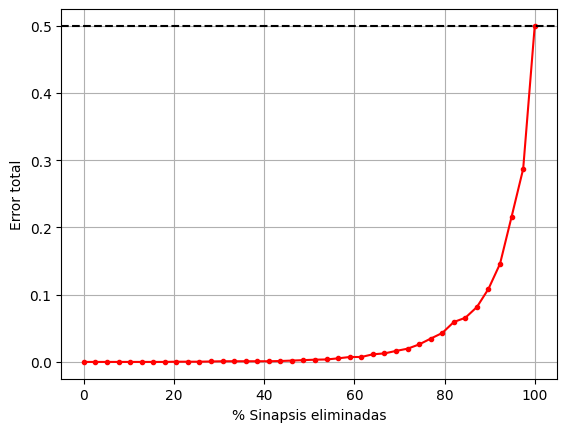
\includegraphics[width=0.7\textwidth]{img_informe/error_sinapsis_borrada.png}
	\caption{Error total en función del procentaje de sinapsis borradas.}
	\label{fig:error_sinapsis}
\end{figure}

\subsection{Capacidad frente a pérdida de sinapsis}

Por otro lado, se analizó también como evoluciona la capacidad de la red ante el borrado de pesos de la matriz. Se puso a disposición de la red 120 patrones, ya que es un valor cercano al máximo teórico del mayor umbral en la tabla~\ref{tab:teorica_hertz}. En la figura~\ref{fig:cap_sin} se puede observar la evolución mencionada para los distintos umbrales de tolerancia usados en el ejercicio de la sección~\ref{sec:ej2}. El comportamiento es acorde al que se podría predecir. La capadidad en cada caso baja cuasi linealmente.


\begin{figure}[htpb!]
	\centering
	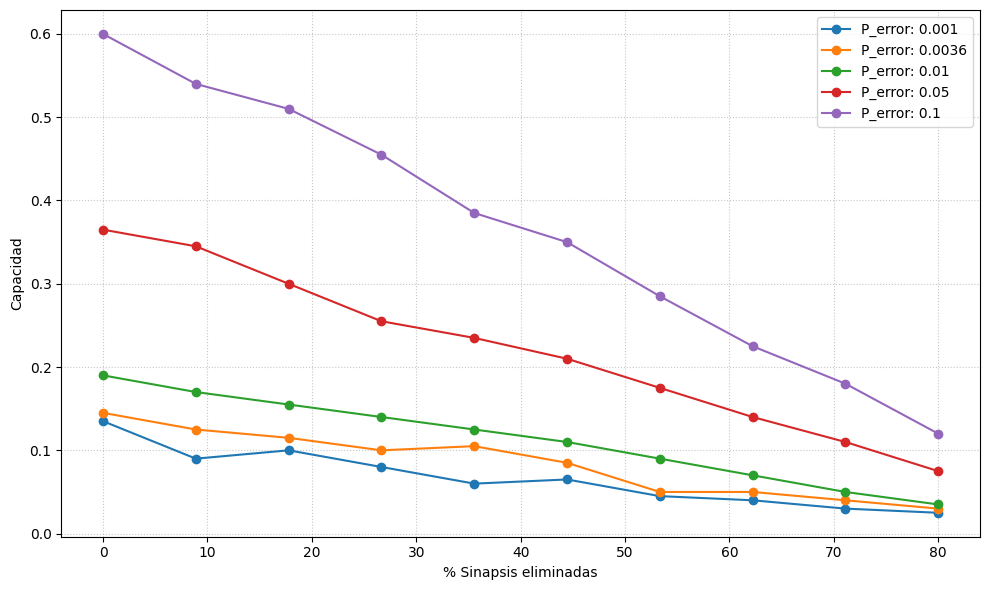
\includegraphics[width=0.7\textwidth]{img_informe/capacidad_sinapsis_borradas.png}
	\caption{Capacidad en función del procentaje de sinapsis borradas.}
	\label{fig:cap_sin}
\end{figure}

\subsection{Energía ante actualización asincrónica}

Para este último paso, se experimentó con la función Energía. Se definió una red y se la entrenó con 15 patrones. Posteriormente, se fue alterando la matriz de pesos de la red en distintas medidas para observar que pasaba al pedirle que devuelva uno de los patrones (con un ruido de $30\%$) con los que fue entrenada. En la figura~\ref{fig:energia} se observa como cada versión de la red evoluciona a lo largo de las épocas. Por otro lado, en el cuadro subsiguiente se puede observar el error que tuvo cada versión de la red. 

Las dos redes con menos daño lograron reconstruir el patrón sin error. Sin embargo, la red con $20\%$ de daño llegó a un mínimo por debajo del que encontró la red con $40\%$ de daño. Por más de que el estado de las neuronas sea el mismo, como la matriz de pesos es distinta, el paisaje de energía difiere. Sería como decir que ambas encontraron las mismas coordenadas en el paisaje, pero el valle situado en dichas coordenadas es más profundo en una que en la otra.

Para la red con $80\%$ de daño, se observa como el nivel de energía alcanzado es mucho más bajo y además no logró reconstruir el patrón exitosamente. No solo que el valle es mucho menos produndo que en los casos anteriores, sino que está en el lugar incorrecto.

\begin{figure}[htpb!]
	\centering
	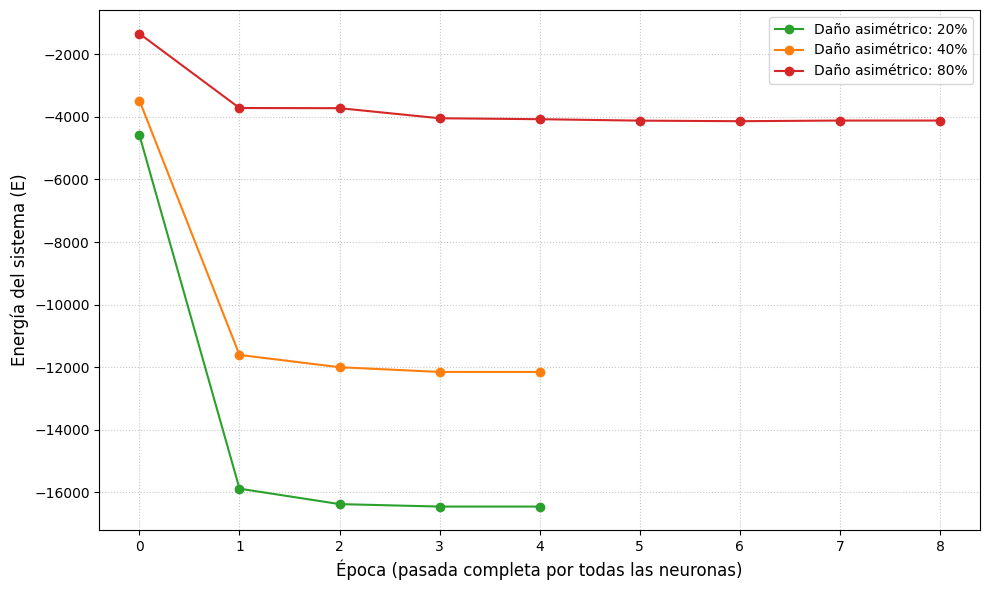
\includegraphics[width=0.7\textwidth]{img_informe/energia_ruido_sinapsis.png}
	\caption{Energía en función de la época.}
	\label{fig:energia}
\end{figure}

\begin{table}[htpb]
	\centering
	\vspace{0.2cm}
	\begin{tabular}{cccc}
		\hline
		\textbf{Daño estructural} & \textbf{Error Final} & \textbf{Píxeles Incorrectos} & \textbf{Épocas de Convergencia} \\
		\hline
		20\% & 0.0\% & 0 & 4 \\
		40\% & 0.0\% & 0 & 4 \\
		80\% & 22.0\% & 44 & 8 \\
		\hline
	\end{tabular}
	\label{tab:asim_dam}
	\caption{Resultados de recuperación ante daño asimétrico (Ruido inicial fijo: 30\%)}
\end{table}